
\stest{
Эдгээрээс аль нь танд чухал вэ?
}{2}{[+]Хэрэглэхэд хялбар//Олон бодлого оруулахад хялбар//Форматыг нь урьдчилан хэлбэржүүлсэн//Математикийн томъёо оруулахад хялбар//Бодолт, хариу, түлхүүрийг хэвлэх горимтой//Бодлого, асуулт, сонгох (нэг болон олон сонголтот) ба нөхөх тестүүдийг дэмждэг//Онооны нийлбэрийг вариант бүрээр автоматаар тооцдог//Вариантыг хүссэн тоогоороо үүсгэх боломжтой//Гадны сургуулийн шалгалтын материал шиг//LaTeX дээр суурилсан//Дурдагдаагүй бусад зүйлс}

%\problem[бодолтын хэсгийн өндрийн хэмжээ]{бодлогын өгүүлбэр}{оноо}{бодолт ба хариу}

\problem[0]{
Бодлого оруулах байдлыг үүгээр харууллаа. Математикийн томъёо $x^2+y^2=1$. $$\frac{x^2}{a^2}+\frac{y^2}{b^2}=1$$ Бодлогын өгүүлбэр дунд
\begin{center}
\begin{tabular}{r|rrr}
  & \multicolumn{3}{c}{$Y$} \\
  $X$  & $-1$ & 0 & 1 \\
  \hline
  $-1$ & 0.2 & 0.2 & 0.1 \\
  0 & 0 & 0.1 & 0.2 \\
  1 & 0 & 0 & 0.2 \\
\end{tabular}
\end{center}
хүснэгт оруулж байна. Харин бодлогын бодолтыг хаана бичиж өгөх вэ?
}{
5
}{
Бодолтыг энд бичиж өгнө.
}

\problem[6]{
\texttt{TikZ} ашиглан зурсан зураг оруулж байна.
\begin{center}
 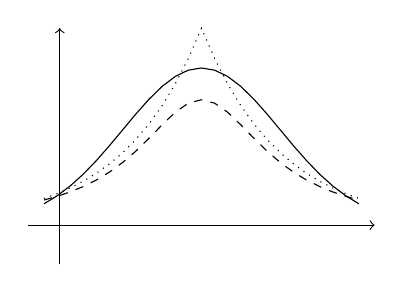
\begin{tikzpicture}[xscale=1,yscale=5]
  \draw[->] (-2.2,0) -- (2.2,0);
  \draw[->] (-1.8,-0.1) -- (-1.8,0.5);
  \draw[] plot[domain=-2:2] (\x,{1/sqrt(2*pi)*exp(-1*\x*\x/2)});
  \draw[dashed] plot[domain=-2:2] (\x,{1/(pi*(1+\x*\x))});
  \draw[dotted] plot[domain=-2:2] (\x,{exp(-sqrt(\x*\x))/2});
 \end{tikzpicture}
\end{center}
Мөн бодолтын хэсгийн өндрийн хэмжээг удирдах боломжтой.
}{
5
}{

}

\begin{lrbox}{\lstListing}
\begin{lstlisting}[language=python]
import random, math                                    # this is comment

c = 2.2039

while True :
  u = random.random()
  y = -1.0 * math.log(random.random())
  if c * u < y * (math.exp(-1.0 * y ** 2 / 2) + y) :   # this line is extra . . . too long
    print y
    break
\end{lstlisting}
\end{lrbox}

\problem[0]{
Програмын эх кодыг ч оруулах боломжийг шийдэж өгсөн. \printlisting Ийм маягаар дурын хэл дээр бичигдсэн програмын эх кодыг оруулах боломжтой. Гэвч энд латинаас бусад үсгээр comment буюу тайлбар бичих боломжгүйг анхаарна уу.
}{
5
}{

}

%\question[хариултын хэсгийн өндрийн хэмжээ]{асуулт}{оноо}{хариу}

\question{
Хариултын хэсгийн хэмжээ тодруулбал өндрийг нь өөрчлөх боломжтой юу?
}{
3
}{
Боломжтой.
}

\question{
Нийт оноог автоматаар тооцоолж гаргадаг уу?
}{
3
}{
Тийм.
}

%\stest{асуулт}{оноо}{сонголт1//[+]зөвсонголт//сонголт3}

\stest{
Сонгох тест оруулах боломжтой юу?
}{2}{[+]Тийм//Үгүй}

%\ptest{асуулт \ehide{томъёо} асуулт \thide{текст, олон мөр дамнахыг дэмжинэ} асуулт}{оноо}

\ptest{
Нөхөх тестийг \thide{ийм} маягаар оруулна.
}{
3
}

\ptest{
Томъёо бүхий нөхөх тестийг $E(2X+Y)=\ehide{2EX}+EY$ байдлаар оруулна.
}{
3
}
